\section{Funciones Meromorfas y el Logaritmo}

\subsection*{Ceros y polos }


%\begin{definition}
%    Dada \(f\in \ho(\Omega)\), \(z_0\in \Omega\) es un \emph{cero} de \(f\) si \(f(z_0) = 0\). %\comentario{Si \(f\not\equiv 0\) sus ceros son isolados, \(\blacksquare\) \hyperlink{thm248}{4.8.}}  
%\end{definition}

\hypertarget{thm311}{}
\begin{theorem}
    \textbf{1.1.} Sean \(\Omega\ab\subset \C\) conexo, \( f \in \ho(\Omega)^\times\) e \(z_0 \in \Omega : f(z_0) = 0\). Entonces, existen \(U\ab \in \U_{z_0}\),  \(!n \in \N \) e \(g \in \ho(U)^\times : f(z) = (z-z_0)^n g(z), \ \forall z \in U\).  
\end{theorem}

\demo{\(\exists U \in \U_{z_0} : 0 \not\equiv f(z)= \sum a_k (z-z_0)^k\). Luego \(\exists n: a_n \neq 0\), así   
\[f(z) = (z-z_0)^n [a_n + a_{n+1}(z-z_0) + \cdots] = (z-z_0)^n g(z).\]
Para la unicidad, si \(f(z) = (z-z_0)^m h(z), \ m>n\), tendríamos \(g(z) = (z-z_0)^{m-n}h(z) \to 0\neq a_n\) cuando \(z \to z_0\), parecido si \(m<n\).\Lightning
}

\begin{definition}
    Sea \(\widehat{\Omega}:= \Omega \setminus \{z_0\} : \Omega\ab \in \U_{z_0} \), \emph{vecindad punteada} de \(z_0 \in \C\).\footnote{Más formalmente seria \(\widehat{B}(z_0;r):= \{z\in \C : 0 < |z-z_0|<r : r >0\}\).} Decimos que \(f\), tiene una \emph{singularidad} \ \(\rotatebox{90}{$|$} \star  \rotatebox{90}{$|$}\) \ en \(z_0\) si fuera holomorfa apenas en  \(\widehat{\Omega}\). 
    \vspace{-0.2cm} 
    \begin{itemize}[left = 1cm, label = \(\star\)]
        \item \emph{Removible} \ \(\leftarrow \exists w \in \C \mid\) si \(f(z_0):= w\), entonces \(f\in \ho(\Omega)\).     
        \item \emph{Polo} \ \(\leftarrow z_0\) es singularidad removible de \(\nicefrac{1}{f}: z_0\mapsto w =0\).% \(\star\) \  \emph{Esencial} e.o.c..
        \item \emph{Esencial} \ \(\leftarrow \) No es removible ni polo. 
    \end{itemize}
\end{definition}

\hypertarget{thm312}{}
\begin{theorem}
    \textbf{1.2.} Si \(f\) tiene un polo en \(z_0\in \Omega\ab \subset \C\), entonces existen \(h \in \ho(\Omega)^\times\) e \(!n \in \N :  f(z ) = (z-z_0)^{-n} h(z)\). \comentario{Sigue del \(\blacksquare\) \hyperlink{thm311}{1.1.} pues \(\nicefrac{1}{f(z)} = (z-z_0)^n g(z)\)}  
\end{theorem}

\begin{note}
    Llamamos a los enteros \(n\) en los \(\blacksquare\) \hyperlink{thm311}{1.1.} e \(\blacksquare\) \hyperlink{thm312}{1.2.} de \emph{orden} del cero u polo, respectivamente, serán \emph{simples} si es que \(n =1 \).
\end{note}

\hypertarget{thm313}{}
\begin{theorem}
    \textbf{1.3.} Si \(f\) tiene un polo de orden \(n \) en \(z_0 \in \Omega\ab \subset \C\), entonces \(\exists U\ab \in \U_{z_0}\) donde
    \[f(z) = \frac{a_{-n}}{(z-z_0)^n} + \frac{a_{-(n-1)}}{(z-z_0)^{n-1}} + \cdots + \frac{a_{-1}}{(z-z_0)}+ G(z): G \in \ho(U).\]
\end{theorem}

\demo{\[f(z) = (z-z_0)^{-n} h(z) = (z-z_0)^{-n} \sum_{k=0}^\infty a_k (z-z_0)^k, \ \ \blacksquare \ \text{\hyperlink{thm312}{1.2.}}.\]
\vspace{-0.2cm}
} 

\begin{note}
    La suma de índices negativos en \(\blacksquare\) \hyperlink{thm313}{1.3.}, \(P(z)\) es llamada \emph{parte principal} de \(f\) en \(z_0\), y \(\operatorname{res}_{z_0}f = a_{-1}\) es el \emph{residuo} de \(f\) en el polo \(z_0\). 
\end{note}

\begin{theorem}
    \textbf{1.4.} Si \(f\) tiene un polo de orden \(n\) en \(z_0\), entonces 
    \[\operatorname{res}_{z_0}f = \lim_{z\to z_0} \frac{1}{(n-1)!} \left(\frac{d}{dz}\right)^{n-1} (z-z_0)^nf(z). \textcolor{gray}{ \ \ \rightarrow \ \blacksquare \ \text{\hyperlink{thm313}{1.3.}}}\]   
\end{theorem}

\vspace{-0.2cm}
\begin{note}
    En la práctica son polos simples, luego \(\operatorname{res}_{z_0}f = \underset{z\to z_0}{\lim}(z-z_0) f(z)\). 
\end{note}

\subsection*{Fórmula del residuo}

\begin{theorem}
    \textbf{2.1.} Sean \(\Omega\ab \in \U_{z_0}\), \(f\) holomorfa en \(\widehat{\Omega}\) con polo en \(z_0 \in D : \overline{D}\subset \Omega\). Entonces, 
    \[\int_{\partial D} f(z) \ dz = 2 \pi i \cdot \operatorname{res}_{z_0}f. \]
\end{theorem}

\demo{
    Combinando la demostración del \(\blacksquare\) \hyperlink{thm241}{4.1.} e la fórmula en \(\blacksquare\) \hyperlink{thm313}{1.3.} tenemos,
    \[\int_{\partial D} f(z) \ dz = \int_{\partial D_\epsilon} f(z) \ dz= 2\pi i \cdot a_{-1}\cdot \frac{1}{2 \pi i }\int_{\partial D_\epsilon} \frac{1}{z-z_0} \ dz =2 \pi i \cdot a_{-1}.\]
    Eso pues en \(f(z) = P(z) + G(z) \) cuasi todo mundo tiene primitiva en \(D_\epsilon\), menos el término en \(P(z)\) asociado a \(k = -1\).      
}

\begin{corollary}
    \textbf{2.3. (\emph{Formula del residuo})} Sean \(\Omega\ab\subset \C\), \(P:= \{z_1, z_2, \ldots , z_N\}\subset \Omega\) polos de \(f\) holomorfa en \(\Omega \setminus P \) e \(P \subset D : \overline{D} \subset \Omega\). Entonces, 
    \[\int_{\partial D} f(z) \ dz = 2\pi i \sum_{k=1}^N \operatorname{res}_{z_k} f. \] 
\end{corollary}

%\ejemplo{
%    \begin{example}
%        \[\int_{-\infty}^{\infty} \frac{1}{1+x^2} \ dx \ \sim \ \int_{\Gamma_R} \frac{1}{1+z^2} \ dz \]
%    \end{example}
%}

\hypertarget{thm331}{}
\begin{theorem}
    \textbf{3.1. (\emph{Riemann})} Sean \(\Omega\ab \in \U_{z_0}\) e \(f\) holomorfa e limitada en \(\widehat{\Omega}\). Entonces, \(z_0\) es singularidad removible. 
\end{theorem}

\demo{
    \parbox[a]{0.25\textwidth}{\- }
    \parbox[b]{0.7\textwidth}{
    \[f(z) = \frac{1}{2 \pi i }\int_{\partial D} \frac{f(\zeta)}{\zeta - z} \ d\zeta = \int_0^{2\pi} g(z, s) \ ds =: F(z).\] 
    Del \(\blacksquare\) \hyperlink{thm354}{5.4.} \(F \in \ho(\Omega)\). Muestra que la fórmula vale para \(z \neq z_0\), replicando la demostración del \(\blacksquare\) \hyperlink{thm241}{4.1.}.
    \vspace{0.5cm}
    }
}

\begin{textblock*}{6cm}(2.4cm, 22.4cm)
        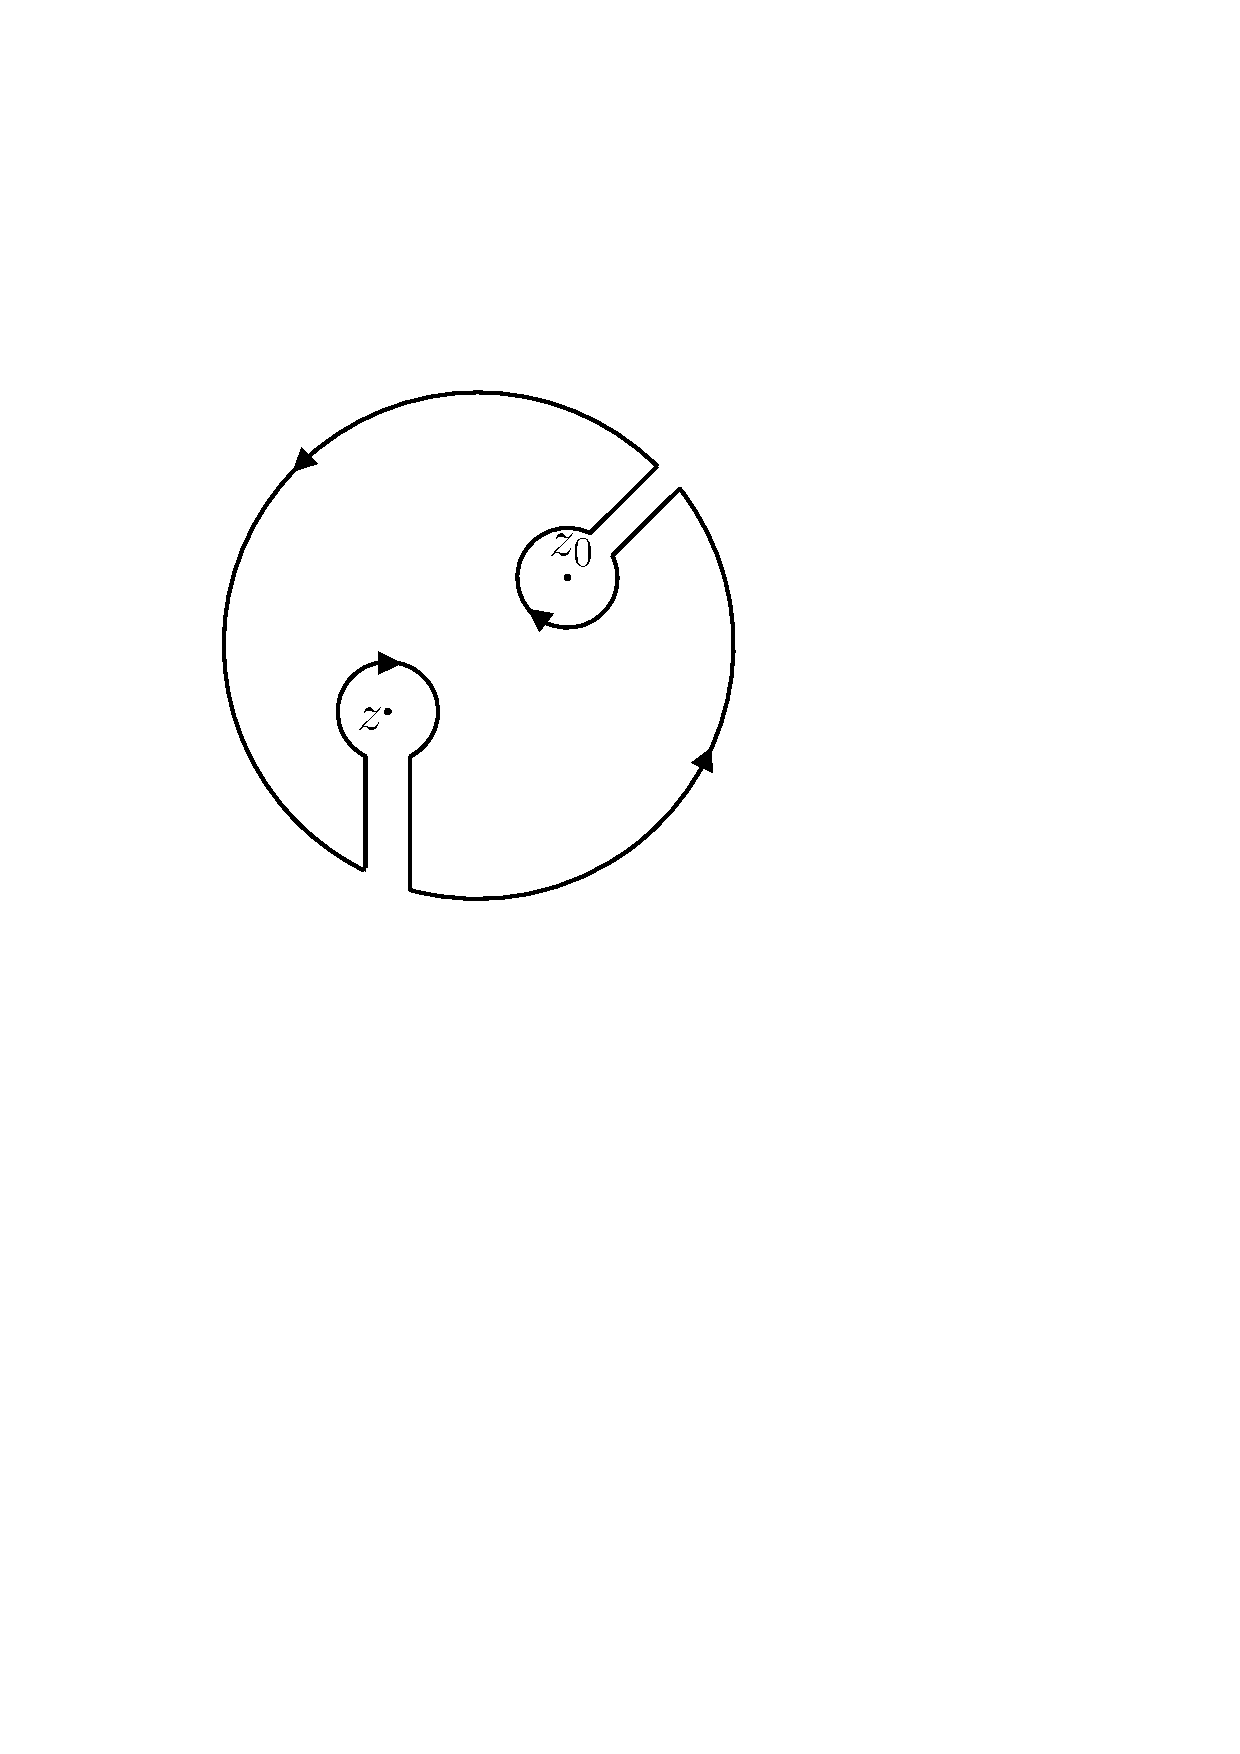
\includegraphics[width = 0.57\linewidth]{Imagens/riemann.pdf}
\end{textblock*}

\begin{corollary}
    \textbf{3.2.} Sean \(\Omega\ab \in \U_{z_0}\) e \(f\) homorfa en \(\widehat{\Omega}\). Entonces, \(f\) tiene un polo en \(z_0 \ \leftrightharpoons \ |f(z)| \to \infty\) cuando \(z\to z_0\). \comentario{Mogollas} 
\end{corollary}

\begin{theorem}
    \textbf{3.3. (\emph{Casorati-Weierstrass})} Sean \(D:= B(z_0; r)\), \(f\) holomorfa en \(\widehat{D}\) e \(z_0\) singularidad esencial de \(f\). Entonces, \(f(\widehat{D})\) es densa en \(\C\). 
\end{theorem}

\demo{Por contradicción, si \(\exists w \in \C\) e \(\delta>0: |g(z)| = |f(z)-w|>\delta, \ \forall z \in \widehat{D}\), entonces \(\nicefrac{1}{g}\) tiene singularidad removible en \(z_0\), \(\blacksquare\) \hyperlink{thm331}{3.1. (\emph{Riemann})}. Si \((\nicefrac{1}{g}) (z_0)\neq 0\), \(f \in \ho(\Omega)\), caso contrário \(f\) tendría un polo en \(z_0\).\Lightning
%\[|g(z)| = \left|\frac{1}{f(z) - w}\right| < \frac{1}{\delta} \ \leftrightharpoons \ g\text{ tiene singularidad removible en }z_0.\]
%Si \(g(z_0) \neq 0\) \(f \in \ho(\Omega)\), caso contrário \(f\) tendría un polo en \(z_0\).\Lightning 
}

\begin{definition}
    Sean \(\Omega\ab\subset \C\) e \(P:= \{z_1, z_2, \ldots , z_N\}\subset \Omega\). Decimos que \(f\) es \emph{meromorfa} en \(\Omega\) si (i) \(f\) es holomorfa en \(\Omega \setminus P \) e (ii) \(z_j \in P\) es polo de \(f, \ \forall j\leq N\).     
\end{definition}

\begin{definition}
    Llamamos \emph{esfera de Riemann} a \(\C \cup \{\infty\} =: \C^*\simeq \E^2\).\footnote{Compactificación de Alexandroff de \(\C \simeq \R^2\).} La analíticidad de \(f(z)\) en \(\infty\) se va a corresponder con la analíticidad de \(F(z) := f(\nicefrac{1}{z})\) en \(z= 0\).     
\end{definition}

\begin{theorem}
    \textbf{3.4.} Las funciones meromorfas en \(\C^*\) son funciones racionales. 
\end{theorem}

\demo{\(f\) tiene finitos polos \(\{z_1, \ldots, z_n\}\subset \C^*\) (compacto). Escriba \(f(z) = P_k(z) + G_k(z)\) (en \(U_k \in \U_{z_k}\)) e \(f(\nicefrac{1}{z}) = \widetilde{P}_\infty(z) + \widetilde{G}_\infty (z)\) (en \(U_0 \in \U_0\)). Muestre que \(H(z) := f(z)- \widetilde{P}_\infty(\nicefrac{1}{z}) - \sum P_k(z)\) es entera limitada, \(\blacksquare\) \hyperlink{coro45}{4.5. (\emph{Liouville})}. 
}

\subsection*{Principio del Argumento y Aplicaciones}

\begin{theorem}
    \textbf{4.1. (\emph{Principio del Argumento})} Sean \(f\) meromorfa en \(\Omega\ab\subset \C\) e \(\gamma \subset \Omega\) una curva cerrada. Si \(f\) no tiene ceros ni polos en \(\gamma\), entonces: %  \(Z:= \#\{z \in \Omega : f(z)= 0 \}\) e \(P:=\#\{z_j \in \Omega : z_j \text{ es polo}\}\). ,  
    \[\int_{\gamma} \frac{f'(z)}{f(z)} \ dz = Z - P, \]
    donde \(Z\) e \(P\) son la cantidad de ceros e polos de \(f\) dentro de \(\gamma\) (con multiplicidad). 
\end{theorem}

\demo{Si \(f(z) = (z-z_0)^n g(z)\) en \(U \in \U_{z_0} : f(z) \neq 0 \) en \(\widehat{U}\), entonces \(\nicefrac{f'}{f} = \nicefrac{n}{z-z_0} + \nicefrac{g'}{g} \), polo simple de residúo \(n\). Analogamente pasa con los polos, pronto.  }

\hypertarget{thm343}{}
\begin{theorem}
    \textbf{4.3. (\emph{Rouché})} Sean \(f, g \in \ho(\Omega)\) e \(D : \overline{D} \subset \Omega\ab \). Si \(|f(z)| > |g(z)|, \ \forall z \in \partial D\), entonces \(f \) e \(f+g\) tienen misma cantidad de ceros en \(D\).
\end{theorem}

\demo{\(f_t := g + t f, \ \forall t \in [0,1]\) no tiene ceros en \(\partial D\). Muestra que \(n_t := \nicefrac{1}{2\pi i} \int_{\partial D} \ \nicefrac{f_t'}{f_t} \ dz \) es constante, \(\blacksquare\) (\emph{TVM - \(\R\)}), contínua en \(t\), luego \(n_0 = n_1\), pronto. }

\hypertarget{thm344}{}
\begin{theorem}
    \textbf{4.4. (\emph{Aplicación Abierta})} Si \(f \in \ho(\Omega)\setminus \C\), entonces \(f\) es abierta.
\end{theorem}

\demo{Sean \(w_0 = f(z_0)\), \(\delta>0 :\overline{D_\delta} := B[z_0;\delta] \subset \Omega\) e \(f(z) \neq w_0\) en \(\partial D_\delta\), también 
\[g(z) := f(z) - w = (f(z) -w_0) + (w_0 - w)=  F(z) + G(z).\]
Siendo \(\epsilon>0 : |f(z) - w_0| \geq \epsilon \) en \(\partial D_\delta \), si \(|w - w_0| < \epsilon \), \(|F(z)| > |G(z)|\) en \(\partial D_\delta\), y el resultado sigue del \(\blacksquare\) \hyperlink{thm343}{4.3. (\emph{Rouché})}. }

\hypertarget{thm345}{}
\begin{theorem}
    \textbf{4.5. (\emph{Principio del Módulo Máximo})} Si \(f \in \ho(\Omega) \setminus \C\), entonces \(\nexists z_0 \in \Omega : |f(z_0)| \geq \ \underset{z \in \Omega}{\sup} \ |f(z)|\). \comentario{\(f( B(z_0;\epsilon) ) \ab\), \(\blacksquare\) \hyperlink{thm344}{4.4. (\emph{AA})}, luego \(\exists z \in D : |f(z)| > |f(z_0)|\) }
\end{theorem}

\begin{corollary}
    \textbf{4.6.} Si \(\Omega\ab\subset \C\) es relativamente compacto e \(f \in \ho(\Omega)\) es continua en \(\overline{\Omega}\), entonces \(\underset{z \in \Omega}{\sup} \ |f(z)| \leq \ \underset{z\in \partial \Omega}{\sup} \ |f(z)|\). \comentario{\(\blacksquare\) (\emph{Bolzano-Weierstrass}) + \(\blacksquare\) \hyperlink{thm345}{4.5. (\emph{PMM})}}   
\end{corollary}

\subsection*{Homotopía y Dominios Simplemente Conexos}

\begin{definition}
    Dos curvas \(\gamma_1, \gamma_2: [a,b] \to \Omega\ab \subset \C \ \mid \ \gamma_1(a) = \alpha = \gamma_2(a)\) e \(\gamma_1(b) = \beta = \gamma_2(b)\) son \emph{homotópicas}, \(\gamma_1 \simeq \gamma_2\), se \(\exists H : [0,1] \times [a,b] \to \Omega\) continua tal que:   
    \[\text{i.} \ \Big|\begin{array}{l}
    H(s,a) = \alpha\\ 
    H(s,b) = \beta
    \end{array}, \ \forall s \in [0,1] \text{ \hspace{1cm} e \hspace{1cm} } \text{ii.} \ \Big| \begin{array}{l}
        H(0,t) = \gamma_1(t)\\ 
        H(1,t) = \gamma_2(t)
    \end{array}, \ \forall t \in [a,b]\]
\end{definition}

\begin{theorem}
    \textbf{5.1.} Si \(f \in \ho(\Omega)\) e \(\gamma_1 \simeq \gamma_2 \) en \(\Omega\), entonces \(\displaystyle \int_{\gamma_1 } f(z) \ dz = \int_{\gamma_2} f(z) \ dz\). \comentario{No admite resumen, véase \cite[pag. 93]{stein}}
\end{theorem}

\begin{definition}
    \(\Omega \subset \C\) es \emph{simplemente conexo} si \(\forall \gamma_1, \gamma_2 : [a,b] \to \Omega \ \mid \ \gamma_1(a) = \alpha = \gamma_2(a) \)  e \(\gamma_1(a) = \beta = \gamma_2(b)\) se tiene que \(\gamma_1 \simeq \gamma_2\) en \(\Omega\). 
\end{definition}

\hypertarget{thm352}{}
\begin{theorem}
    \textbf{5.2.} Toda función holomorfa en dominio simplemente conexo admite primitiva. 
\end{theorem}

\demo{Sean \(z_0 \in \Omega \), \(\gamma: z_0 \leadsto z\), \(F(z) := \int_\gamma f(w) \ dw\) (no depende de \(\gamma\), \(\blacksquare\) \hyperlink{thm351}{5.1.}) e \(\eta: z \leadsto z+h\). Copie el argumento del \(\blacksquare\) \hyperlink{thm221}{2.1.} para ver que
\[F(z+h) -F(z) = \int_\eta f(w) \ dw \hspace{0.5cm} \text{e} \hspace{0.5cm} \lim_{h\to 0}\frac{F(z+h) -F(z)}{h} = f(z). \]}

\begin{corollary}
    \textbf{5.3.} Si \(f \in \ho(\Omega)\) con \(\Omega\ab\subset \C\) simplemente conexo, entonces \(\int_\gamma f(z) \ dz = 0, \ \forall \gamma \subset \Omega\) curva cerrada.  \comentario{Mogollas, directo del \(\blacksquare\) \hyperlink{thm352}{5.2.}} 
\end{corollary}

\subsection*{El Logaritmo Complejo}

\begin{theorem}
    \textbf{6.1.} Sean \(\Omega\ab\subset \C\) simplemente conexo \(: 1 \in \Omega\) e \(0\notin \Omega \). Entonces, \(\exists F \in \ho(\Omega)\), \emph{rama} de \(\log\), esto es, \(F(z) = \log_\Omega(z):= \log |z| + i \arg(z)\) tal que,    
    \vspace{-0.3cm}
    \begin{enumerate}[label = \roman*., left = 1cm]
        \item \(e^{F(z)} = z, \ \forall z \in \Omega\). \hfill ii. \ \(F(r) = \log r, \ r \in \R : |r-1| < \epsilon\).  \hspace{1cm} \-
    \end{enumerate}
\end{theorem}

\demo{Copia la demostración del \(\blacksquare\) \hyperlink{thm352}{5.2.} con \(f(z)= \nicefrac{1}{z}\) e \(\gamma: 1 \leadsto z\); (i) Muestra que \(ze^{-F(z)} = 1\), derivando el lado izquierdo e (ii) \(F(r) = \int_1^r \nicefrac{1}{x} \ dx = \log r\).   }

\ejemplo{\centering \emph{Rama Principal de Logaritmo}
\tcblower
\[\log : \begin{array}{ll}
\C \setminus (-\infty, 0] &\to \hspace{1cm} \C  \\ 
\hspace{1cm}re^{i\theta} &\mapsto \ \ \log r + i\theta 
\end{array}, \hspace{0.5cm} |\theta| < \pi.\]
}

\begin{theorem}
    \textbf{6.2.} Sea \(\Omega\ab \subset \C\) simplemente conexo. Si \(f \in \ho(\Omega)\) e \(f(z) \neq 0, \ \forall z \in \Omega \), entonces \(\exists g \in \ho(\Omega) : f(z) = \exp({g(z)}) \textcolor{gray}{ \ \sim g = \log f}\). 
\end{theorem}

\demo{Defina \(g(z) := \int_\gamma \nicefrac{f'(w)}{f(w)} \ dw + c_0\), onde \(\gamma: z_0 \leadsto z\) e \(c_0 \in\C : e^{c_0} = f(z_0)\). Ahí \(g' = \nicefrac{f'}{f}\) e derivado \(f(z)\exp(-g(z))\) vemos que es constante igual a \( 1\), pronto.  }